\newcommand{\bssid}{\mathbf{B}}
\newcommand{\ssid}{\mathrm{SSID}}
\newcommand{\ssim}{\mathrm{sim}}
\renewcommand{\SS}{\mathbf{S}}
\newcommand{\RR}{\mathbf{R}}
\newcommand{\FF}{\mathbf{F}}
\newcommand{\LL}{\mathbf{L}}
\newcommand{\lleft}{\mathrm{left}}
\newcommand{\rright}{\mathrm{right}}
\newcommand{\RRR}{\hspace{0.4cm}}

\section{Movement Segmentation}

\label{sec:movement}

We study the problem of online processing of WiFi scans collected by a mobile
device.  We refer to each scan as a {\em reading}.
A reading is defined as $\left<t(r), \bssid(r), \ssid, s(\cdot|r)\right>$ where $t(r)$ is
the timestamp of the reading, and $\bssid(r)\subseteq\mathrm{BSSID}$ is a set of
BSSID of the wifi hotspots that the scan detected. 
The $\ssid:\bssid(r)\to\mathrm{Names}$ is a mapping of BSSID names to
user-defined name of the WiFi hotspot.  $s(\cdot|r):\bssid(r)\to R^+$ is a
mapping of BSSID of the reading $r$ to a signal strength; $s(b|r)$ is the
intensity of $b$ in the reading $r$.

\subsection{Movement detection}

In this section we describe an online algorithm to organize the timeline of
readings into multiresolution segments.  The timeline is partitioned such that
within each segment, 

\begin{definition}
    A {\em timeline} $T$ is a sequence of readings.  
    We denote $T_i$ as the $i$-th reading of the timeline $T$.

    A {\em segment} of the timeline $S$ is a contiguous subsequence of $T$.
\end{definition}

The $\bssid(T_i)$ induces a similarity measure among the readings.

\begin{definition}[Reading similarity]
$$\ssim(T_i, T_j) = \mathrm{Jaccard}(\bssid(T_i), \bssid(T_j))
= \frac{|\bssid(T_i) \cap \bssid(T_j)|}{|\bssid(T_i) \cup \bssid(T_j)|}
$$
\end{definition}

This allows us to organize $T$ using hierarchical clustering.
Unlike the traditional hierarchical clustering of sets of items with a
similarity measure, clustering a timeline has the added constraint that each
cluster must only contain adjacent readings.
Algorithm~\ref{alg:bottom-up} is an
adaptation of the bottom-up agglomerative to compute hierarchical timeline
clustering.  In $\mathbf{TimelineClustering}(T)$, 
$\mathbf{merge}(T_i, T_{i+1})$ creates a new node in the hierarchical timeline,
and its BSSID set is simply the union of the BSSID sets of its children:
$$\bssid(\mathbf{merge}(x, y)) = \bssid(x)\cup\bssid(y)$$ 

\begin{algorithm}[t]
    \centering
\begin{tabular}{|l|}\hline
    func {\bf TimelineClustering}($T$) \\\hline
    $X = T$ \\
    {\bf while} $|X| > 1$ \{ \\
        \RRR $i^* = \mathrm{argmax}\{\ssim(T_i,T_{i+1}) : i\in [1, |X|]\}$ \\
        \RRR $r = \mathbf{merge}(T_i, T_j)$ \\
        \RRR $X = \mathbf{replace}\ [T_i, T_{i+1}]\ \mathbf{with}\ r$\\
    \}\\ 
    {\bf return} Tree with root $X$\\ \hline
\end{tabular}
\vspace{0.5cm}
\caption{Bottom-up timeline clustering}
\label{alg:bottom-up}
\end{algorithm}

We remark that {\bf TimelineClustering} is certainly {\em not} an online
algorithm, as it requires $\mathcal{O}(|T|^2)$ complexity to build the
hierarchy.  This will be remedied later by the online version to be presented
later.

Let $H = \mathbf{TimelineClustering}(T)$, where $H$ is a binary tree with the
leaf nodes as the readings in $T$.
$H$ presents a multiresolution segmentation.

We use the following notations:

\begin{itemize}
    \item The leaf-nodes of $H$, written $\mathrm{leaf}(H)$, is just the
        readings $T$.  The nodes of $H$ is writtn $\mathrm{Nodes}(H)$.
    \item The descendants of $v\in \mathrm{Nodes}(H)$ is written
        $\mathrm{descendants}(v)$.
    \item The readings of $v$ is defined as:
        $$\RR(v) = \mathrm{descendants}(v)\cap\mathrm{leaf}(H)$$
    \item Since $H$ is a binary tree, each interior node $v$ has two children,
        written $\lleft(v)$ and $\rright(v)$.
\end{itemize}
level of $v$.

The challenge is the determine the nodes in $H$ whose readings are all at the
{\em same} physical location.  This is determined by the {\em minimum
similarity}.

\begin{definition}[Minimum Similarity]
    Given a set, $R$, of readings, the minimum similarity of $R$, written
    $\mathrm{minsim}(R)$ is defined as:

    $$\mathrm{minsim}(R) = \min\{\ssim(r,r'): (r,r')\in R\times R\}$$
    \label{def:minsim}
\end{definition}

The $\mathrm{minsim}$ provides a measure if a set of readings $R$ span over more
than one physical location.
We observe that if $R$ contains readings taken from two distinct physical
locations, then, due to the spatial distance there will be at least one pair of
readings, $r$ and $r'$, that are quite dissimilar: $\ssim(r, r') \leq \epsilon$ for some
small constant $\epsilon\ll 1$.  This means that $\mathrm{minsim}(R)\leq \epsilon$.

For nodes in the hierarchy, $v\in\mathrm{Nodes}(H)$, its minsim is simply the
minsim of its readings.

\begin{definition}[Minsim for nodes]
    $$\mathrm{minsim}(v) = \mathrm{minsim}(\RR(v))$$
\end{definition}

We will use $\mathrm{minsim}$ and $\epsilon$ to perform the segmentation of $T$
using the hierarchy $H$.  Algorithm~\ref{alg:segments} performs a top-down
traversal of $H$ to identify the top-most nodes in $H$ with 
$\mathrm{minsim}(R) > \epsilon$, which we call {\em homogeneous nodes}.

\begin{algorithm}[t]
    \centering
    \begin{tabular}{|l|}\hline
        func Segments$(v, \epsilon)$ \\ \hline
        if $\mathrm{minsim}(v) > \epsilon$ \{ \\
        \RRR return [$v$] \\
        \} else \{ \\
        \RRR return $\mathrm{Segments}(\mathrm{left}(v), \epsilon) \cup
                      \mathrm{Segments}(\mathrm{left}(v), \epsilon)$ \\
        \} \\ \hline
    \end{tabular}
    \vspace{0.4cm}
    \caption{Identifying homogeneous nodes}
    \label{alg:segments}
\end{algorithm}

Each homogeneous node in corresponds to a segment of the timeline in which all
the readings are at the same physical location according to the BSSIDs.

There are two shortcomings with the approach:

\begin{enumerate}
    \item The timeline clustering is not an online algorithm.
    \item The segmentation requires the threshold measure $\epsilon$.
\end{enumerate}

We will address these issues in the coming sections.

\subsection{Online hierarchical timeline clustering}

Our objective is to update a hierarchical timeline cluster $H$ incrementally when
more readings are appended to the timeline $T$.

We define a procedure $\mathrm{update}(H, v_\mathrm{insert}, v_\mathrm{new})$
where $H$ is the timeline cluster to be updated, and we wish to add a new node
$v_\mathrm{new}$ {\em after} the $v_\mathrm{insert}$.

We analyze the behaviour of $\mathrm{update}(\dots)$ by different cases.
Let $H' = \mathrm{update}(H, v_\mathrm{insert}, v_\mathrm{new})$

\begin{itemize}
    \item If $v_\mathrm{insert} = \mathrm{root}(H)$, then
        $H' = \mathrm{newnode}(v_\mathrm{insert}, v_\mathrm{new})$
    \item Otherwise, define $v_\mathrm{parent} = \mathrm{parent}(v)$, and
        $v_\mathrm{prev} = \mathrm{left}(v_\mathrm{parent})$.

        Next week check if $v_\mathrm{new}$ is closer to $v_\mathrm{insert}$ or
        not, compared to $v_\mathrm{prev}$.
        \begin{itemize}
            \item If $\ssim(v_\mathrm{new}, v_\mathrm{insert}) \geq 
                      \ssim(v_\mathrm{insert}, v_\mathrm{prev})$, then
                    we create a new node $v' = \mathrm{newnode}(v_\mathrm{insert},
                    v_\mathrm{new})$, and promote $v_\mathrm{prev}$ to replace
                    $v_\mathrm{parent}$.  Then, we recursively invoke:
                    $$H' = \mathrm{update}(H, v_\mathrm{prev}, v')$$
            \item If $\ssim(v_\mathrm{new}, v_\mathrm{insert})  <
                      \ssim(v_\mathrm{insert}, v_\mathrm{prev})$, then
                    we try to insert $v_\mathrm{new}$ after $v_\mathrm{parent}$.
                    $$H' = \mathrm{update}(H, v_\mathrm{parent}, v_\mathrm{new})$$
        \end{itemize}
\end{itemize}

The online version of the hierarchical timeline clustering is shown in
Algorithm~\ref{alg:online-cluster}.  For each new reading, it updates the
hierarchical timeline $H$ and the homogeneous nodes based on the differences
between the new $H$ and the old $H$.

\begin{algorithm}[t]
    \centering
    \begin{tabular}{|l|}\hline
        func OnlineTimelineCluster($T$) \\ \hline
        $H = \mathrm{Tree}(\mathrm{first}(T))$ \\
        $\SS = \mathrm{Segments}(\mathrm{root}(H), \epsilon)$ \\
        for $r\in T$ \\
        \RRR $T' = \mathrm{update}(T, r)$ \\
        \RRR for each $v\in \mathrm{Nodes}(T') - \mathrm{Nodes}(T)$ \{\\
        \RRR \RRR if $v$ is a top-level homogeneous node in $T'$ \{\\
        \RRR \RRR \RRR $\SS = \SS\cup v$ \\
        \RRR \} \\
        \RRR for each $v\in \mathrm{Nodes}(T) - \mathrm{Nodes}(T')$ \{\\
        \RRR \RRR $\SS = \SS - \{v\}$ \\
        \RRR \} \\ \hline
    \end{tabular}
    \vspace{0.5cm}
    \caption{Online timeline clustering}
    \label{alg:online-cluster}
\end{algorithm}

\subsection{Unsupervised segmentation}

In practice, the WiFi readings will encounter several differen types of {\em
noises}.

\begin{itemize}
    \item False positives - it is possible that a reading will detect one or
        more BSSIDs which are not local to the physical location.  False
        positives may be the result of faulty WiFi scan, or by moving WiFi
        hotspots created by other mobile devices.
    \item False negatives - a reading my miss certain BSSIDs which are local to
        the physical location.  This may be the result of signal blockage or
        momentary interference.
    \item Moving BSSIDs - moving mobile devices often create transient WiFi
        hotspots, making it possible for a common WiFi BSSID appear at multiple
        physical locations.
\end{itemize}

By choosing the right threshold during the segmentation $\epsilon$, we can eject
errors due to noise.  With the right choice of
$\epsilon$, we classify readings with sufficient difference (as low similarity
between their BSSID sets) as distinct locations even if some readings contain
errorenous BSSIDs.

We make the assumption that all the segments in $H$ are either homogeneous or
not.  At the leaf level, we have $\mathrm{minsim}(v) = 1$, and as we traverse
upwards toward the root, $\mathrm{minsim}(v)\to 0$.  A sudden drop in minsim
from level $i$ to $i+1$ suggests that at the higher level (and coarser timeline
partition), nodes are covering more than one physical location.

The selection of $\epsilon$ is $\mathrm{minsim}$ corresponding to the level with
the largest drop in average $\mathrm{minsim}(v)$ for $v$ in the level.

\subsection{Approximate segmentation using sampling}

The definition of minsim (Definition~\ref{def:minsim}) can be costly as it
requires computation in $\mathcal{O}(|R|^2)$.  As we compute the root node in
the hierarchical timeline, $|R|$ grows rapidly.

Given a node in the hierarchy $H$, We can accurately estimate
$\mathrm{minsim}(v)$ using sampling as follows.

\begin{itemize}
    \item $v_L = \mathrm{left}(v)$, and $v_R = \mathrm{right}(v)$.
    \item Let $R_L = \mathrm{sample}(\RR(v_L), N)$.
    \item Let $R_R = \mathrm{sample}(\RR(v_R), N)$.
    \item Let $\mu = \mathrm{min}\{\ssim(r,r'): r\in R_L, r'\in R_R$
\end{itemize}
Finally the estimation of $\mathrm{minsim}(v)$ is given by:

$$\mathrm{minsim} \simeq \min\{\mathrm{minsim}(v_L), \mathrm{minsim}(v_R), \mu\}$$

\section{Location Identification}

\label{sec:loc}

In Section~\ref{sec:movement}, we described a unsupervised online algorithm to
identify a sequence of movements, $\SS$, based on the BSSID readings.  The result of the
algorithm is a sequence of segments, each of which is guaranteed to be present a
single physical location.

\subsection{Constructing location index}

In this section, we describe an efficient algorithm to identify the set of {\em
unique} locations based on BSSID signatures of each segment.  Given a segment (a
sequence of consecutive readings in the timeline) $S$, $\RR(S)$ is the readings
belonging to $S$, and $\bssid(S) = \bigcup\{\bssid(r): r\in\RR(S)\}$.

The unique locations are characterized by repeated occurrences of segments with
similar BSSID signatures.

While we can use $k$-mean clustering to cluster the segments based on the BSSID
signatures, our application requies an efficient online method that does not
require a prescribed value of $k$.

Recall that the segments $\SS$ is being produced in a streaming fashion.  will
propose an algorithm to incrementally build a database of physical locations
$\LL$.  Each physical location $L\in\LL$ is characterized by a set of {\em
weighted} BSSIDs.

The algorithm begins with an empty set.  As a segment $S$ is generated in $\SS$, we
look for a location $L\in\LL$ that is sufficiently similar $S$ by the measure
of $\ssim(\bssid(L), \bssid(S))$.  If no such $L$ exists, then we have
discovered a new location, and we create a new location in $\LL$ based on $\bssid(S)$.

The algorithm of location identification is given in Algorithm~\ref{alg:loc}.
It has a parameter $c$ which is the minimal similarity for a segment to belong
to a physical location.

\begin{algorithm}[h]
    \centering
\begin{tabular}{|l|} \hline
    func IdentifyLocations$(\SS)$ \\ \hline
    $\LL$ = new index of locations \\
    foreach $S\in\SS$ \{ \\
        \RRR find $L\in\LL$ such that $\ssim(\bssid(L), \bssid(S)) > c$ \\
        \RRR if not found \{ \\
        \RRR \RRR $\LL = \LL\cup \mathrm{newloc}(S)$ \\
        \RRR \} else \{ \\
        \RRR \RRR Update readings of $L$ with readings of $S$ \\
        \RRR \} \\
    \}\\ \hline
\end{tabular}
\vspace{0.4cm}
\caption{Algorithm for identifying distinct locations from a stream of
movements.}
\label{alg:loc}
\end{algorithm}

\subsection{Transient versus persistent locations}

Algorithm~\ref{alg:loc} produces an index of {\em all} locations visited by the
mobile device.  $\LL$ also maintains the association between readings/segments
and the identified physical locations.

Each location $L\in\LL$ has several attributes:
\begin{enumerate}
    \item $\mathrm{freq}(L)$ is the number of times that $L$ appeared in the
        timeline $T$.  This is the number of segments associated to $L$.
    \item $\mathrm{duration}(L)$ is the total duration that the mobile device
        was present at location $L$ in the timeline $T$.  This is the sum of all
        the durations of segments associated to $L$.
\end{enumerate}

The two metrics $\mathrm{freq}(L)$ and $\mathrm{duration}(L)$ allow us to
classify the physical locations into two distinct classes: {\em transcient} and
{\em persistent} locations.

For some minimal duration $\tau$, we can define the transient locations as:
$$\LL_\mathrm{Transient} = \{ L\in \LL :
    \mathrm{freq}(L) = 1\ \mathrm{and}\ \mathrm{duration}(L) < \tau
\}$$

The persistent locations are $\LL_\mathrm{Persistent} = \LL -
\LL_\mathrm{Transient}$.

\section{Semantic Grouping of Physical Locations}

\begin{algorithm}[t]
    \centering
    \begin{tabular}{|l|} \hline
        func merge($\LL$, $K$) \\
        \RRR $\LL$: the locations \\
        \RRR $K$: a set of keywords used to merge locations \\
        \RRR {\em returns}: the set of semantic locations after merging\\ \hline
        $L_\mathrm{new}$ = newlocation($\emptyset$)\\
        foreach $L\in\LL$ \{ \\
            \RRR if $\forall k\in K\ \exists k'\in\ssid(L)\ \mathrm{such\ that}\ k\preceq k'$ \{ \\
            \RRR \RRR $L_\mathrm{new} = L_\mathrm{new}\cup L$ \\
            \RRR \RRR delete $L$ from $\LL$ \\
            \RRR \} \\
        \} \\
        if $L_\mathrm{new}$ is not empty \{ \\
        \RRR $\LL = \LL\cup\{L_\mathrm{new}\}$ \\
        \} \\
        return $\LL$ \\ \hline
    \end{tabular}
    \vspace{0.4cm}
    \caption{Merging locations based on a key SSID set.}
    \label{alg:merge}
\end{algorithm}

\begin{figure*}[t]
    \centering
    \subfigure[]{
        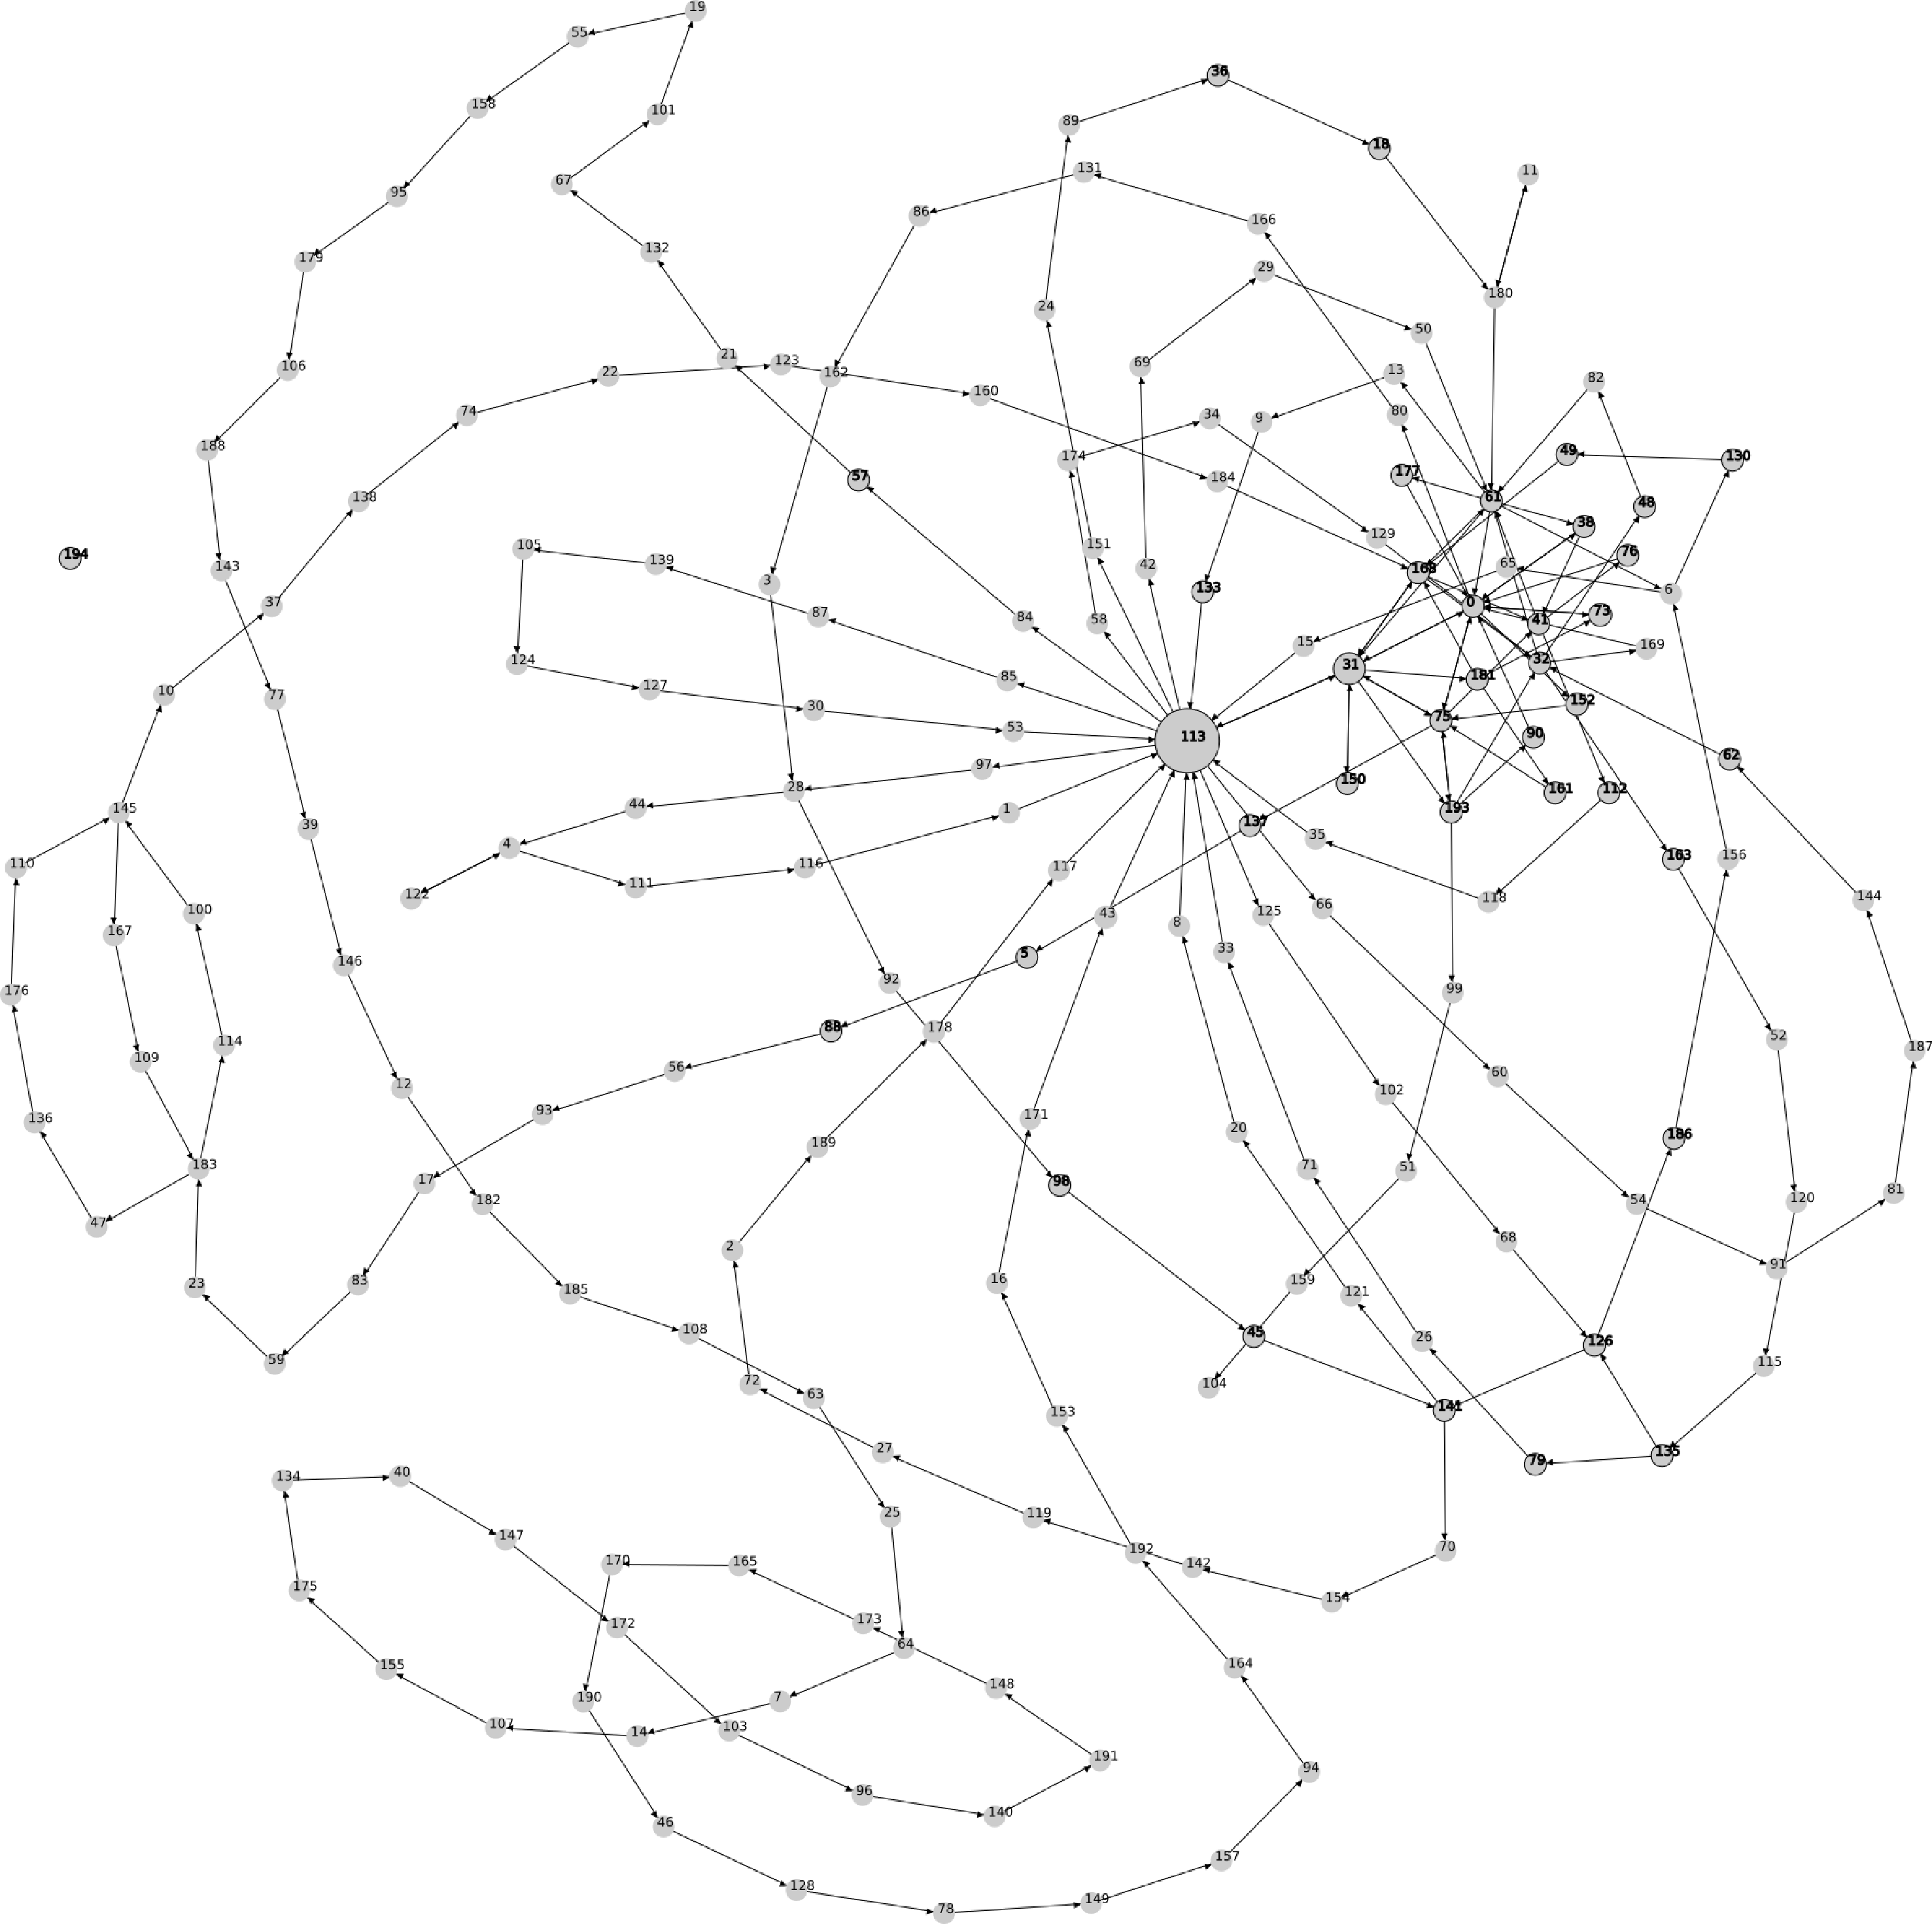
\includegraphics[width=5cm]{../plots/L0.pdf}
    } 
    \subfigure[]{
        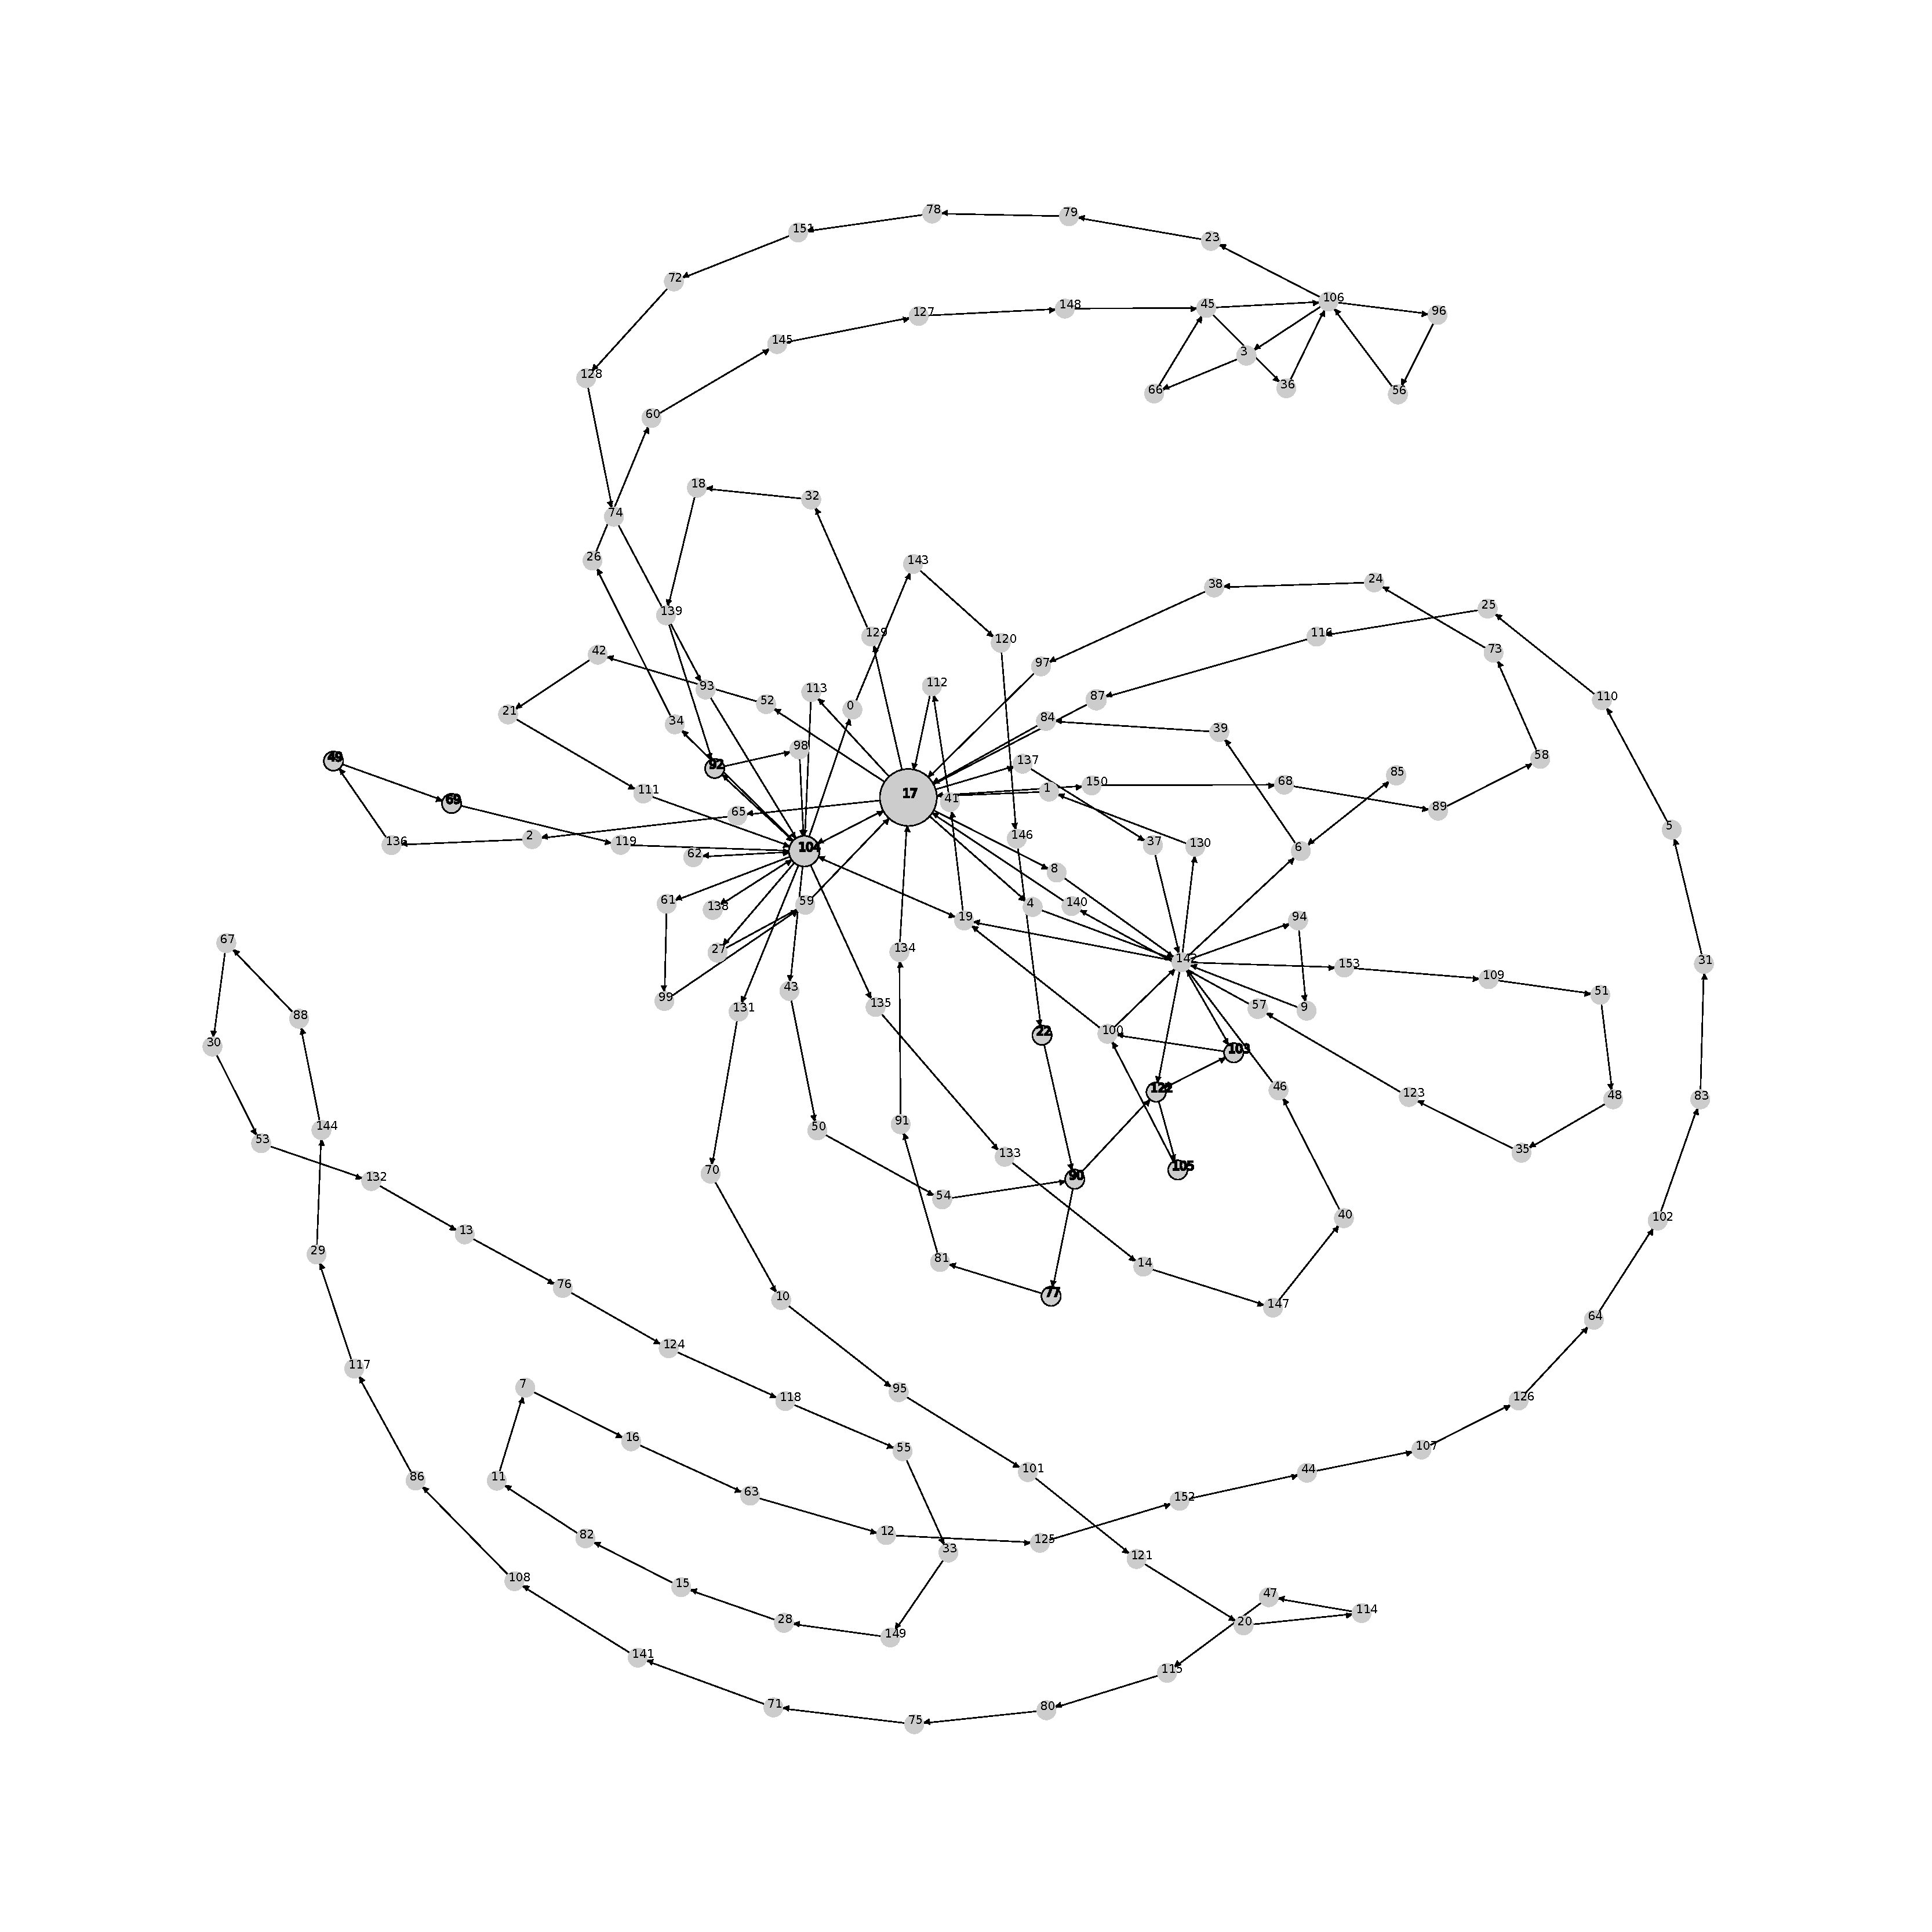
\includegraphics[width=5cm]{../plots/L1.pdf}
    }
    \subfigure[]{
        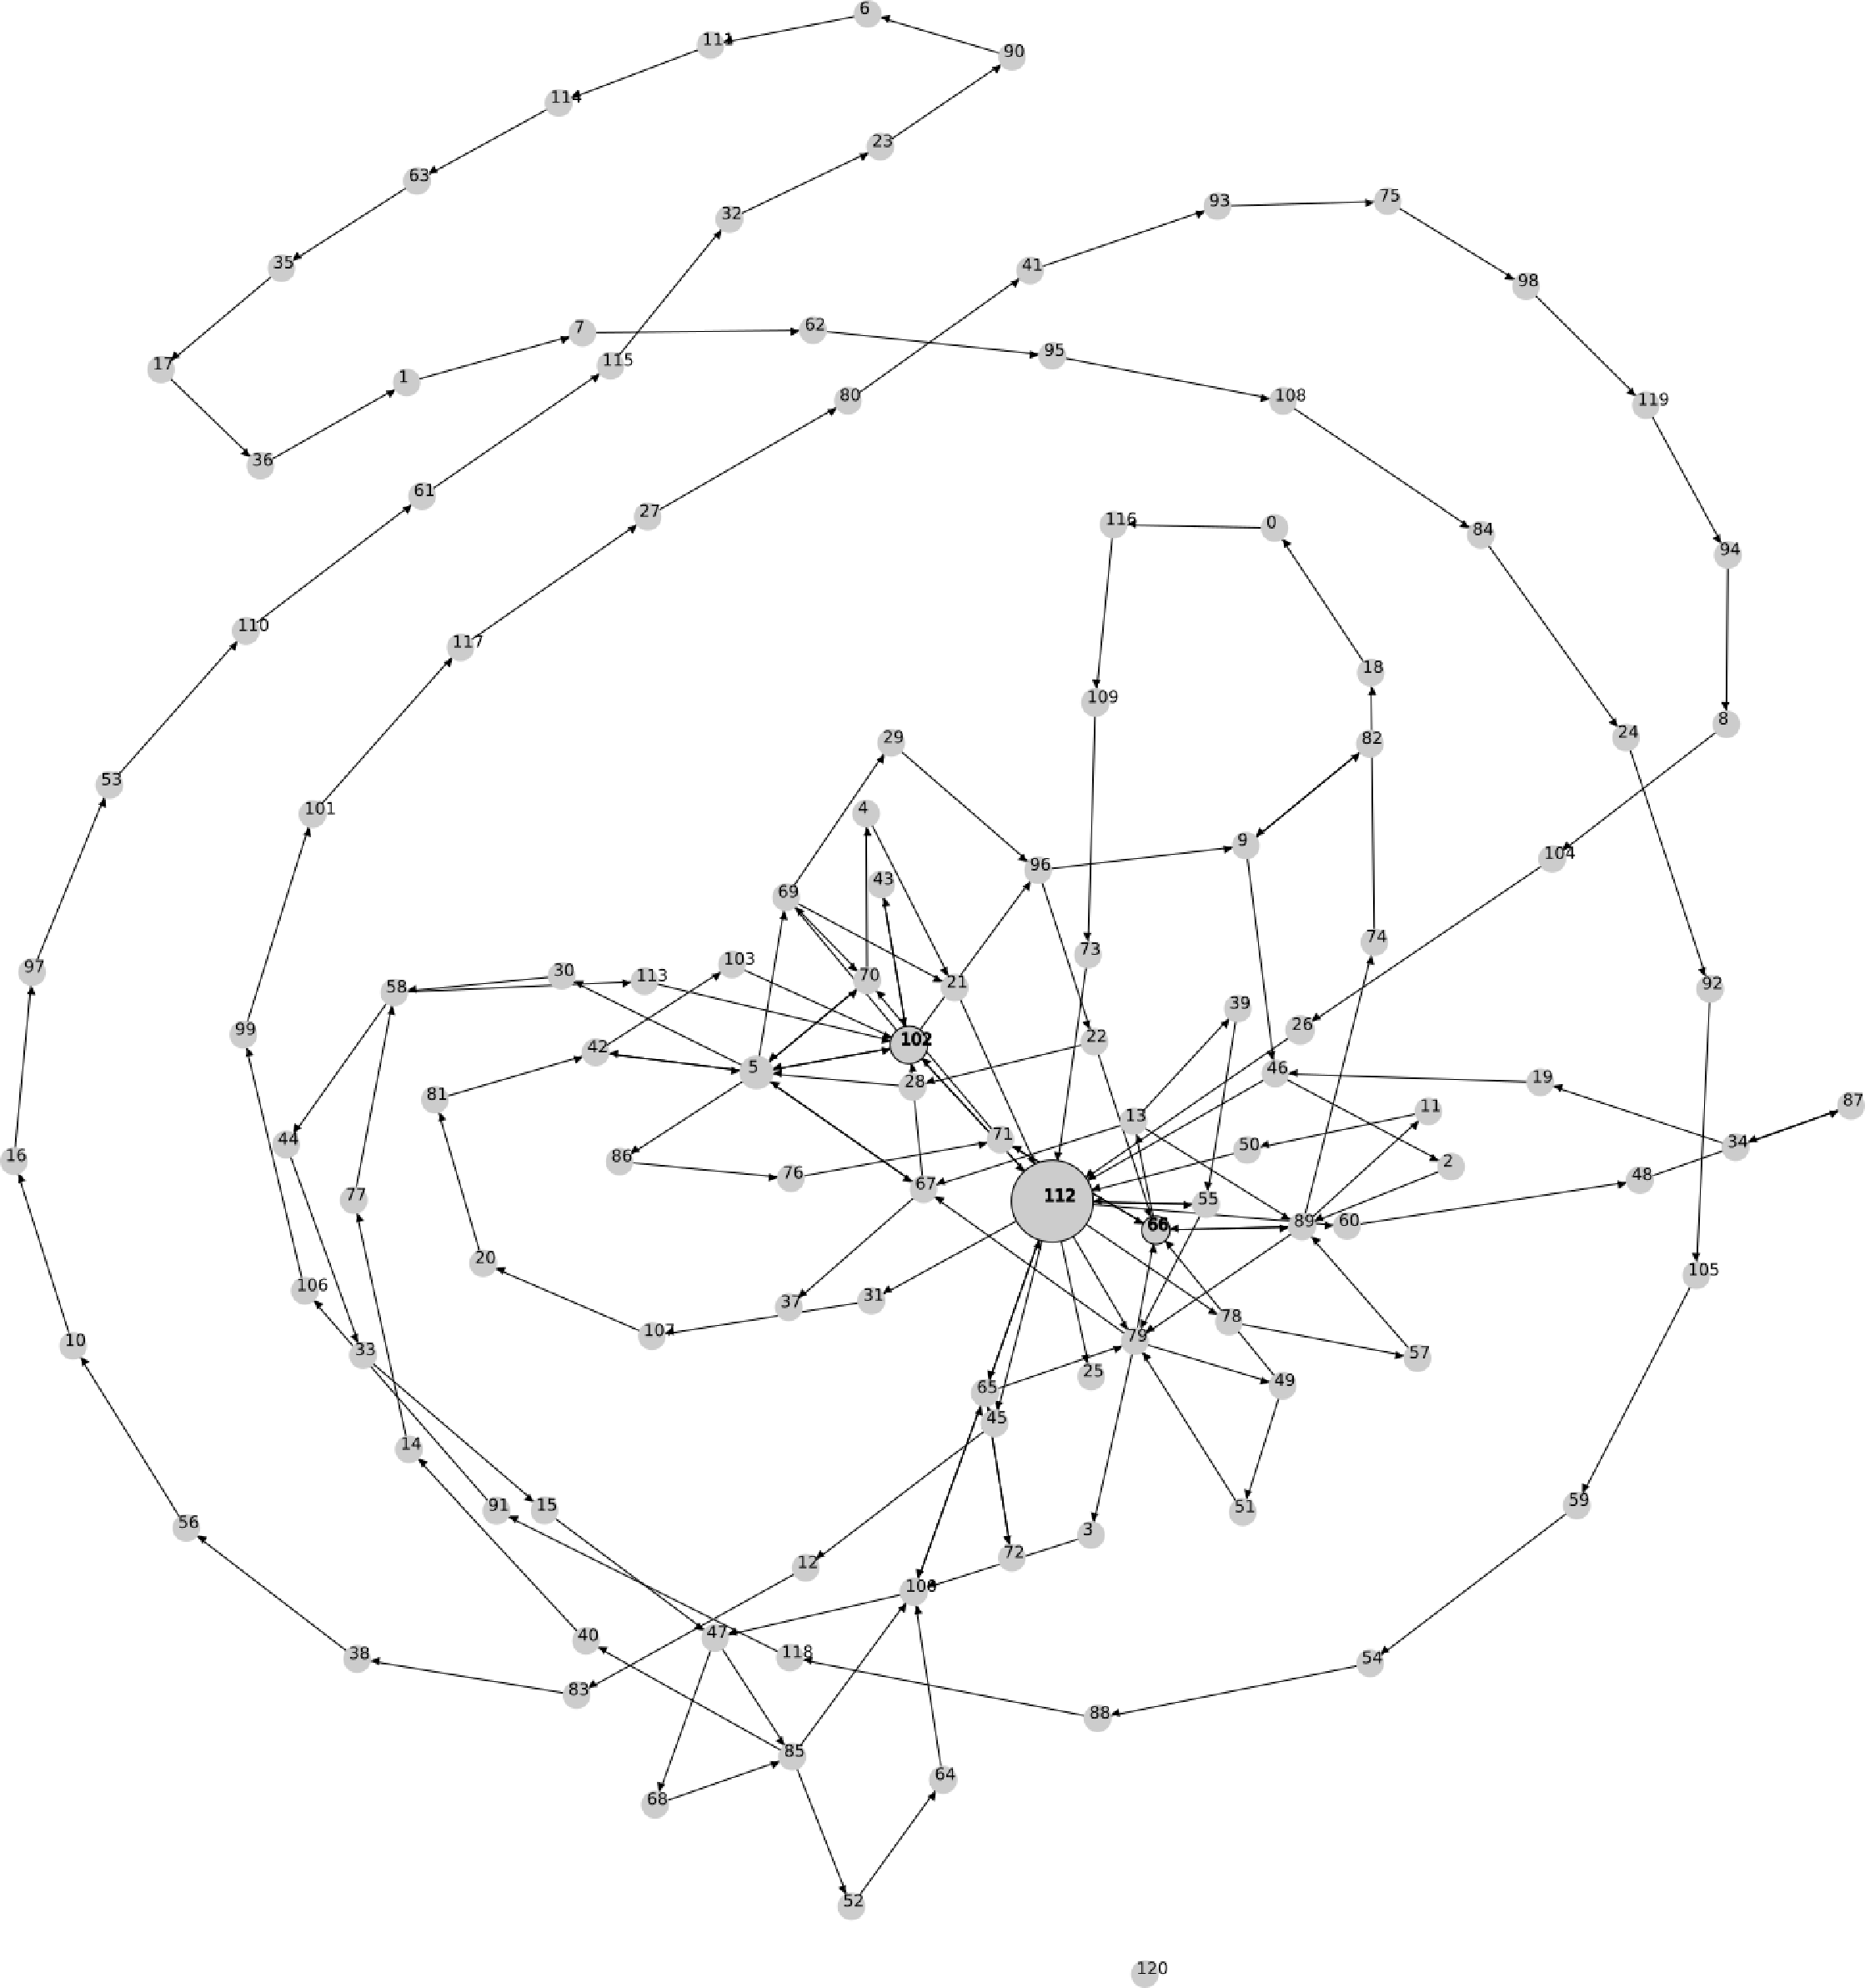
\includegraphics[width=5cm]{../plots/L2.pdf}
    }
    \caption{Transition diagrams of timelines of all locations labeled by: (a)
        physical locations, semantic labels with $i=2$, semantic labels with
        $i=1$.}
\end{figure*}
\begin{figure*}[t]
    \centering
    \subfigure[]{
        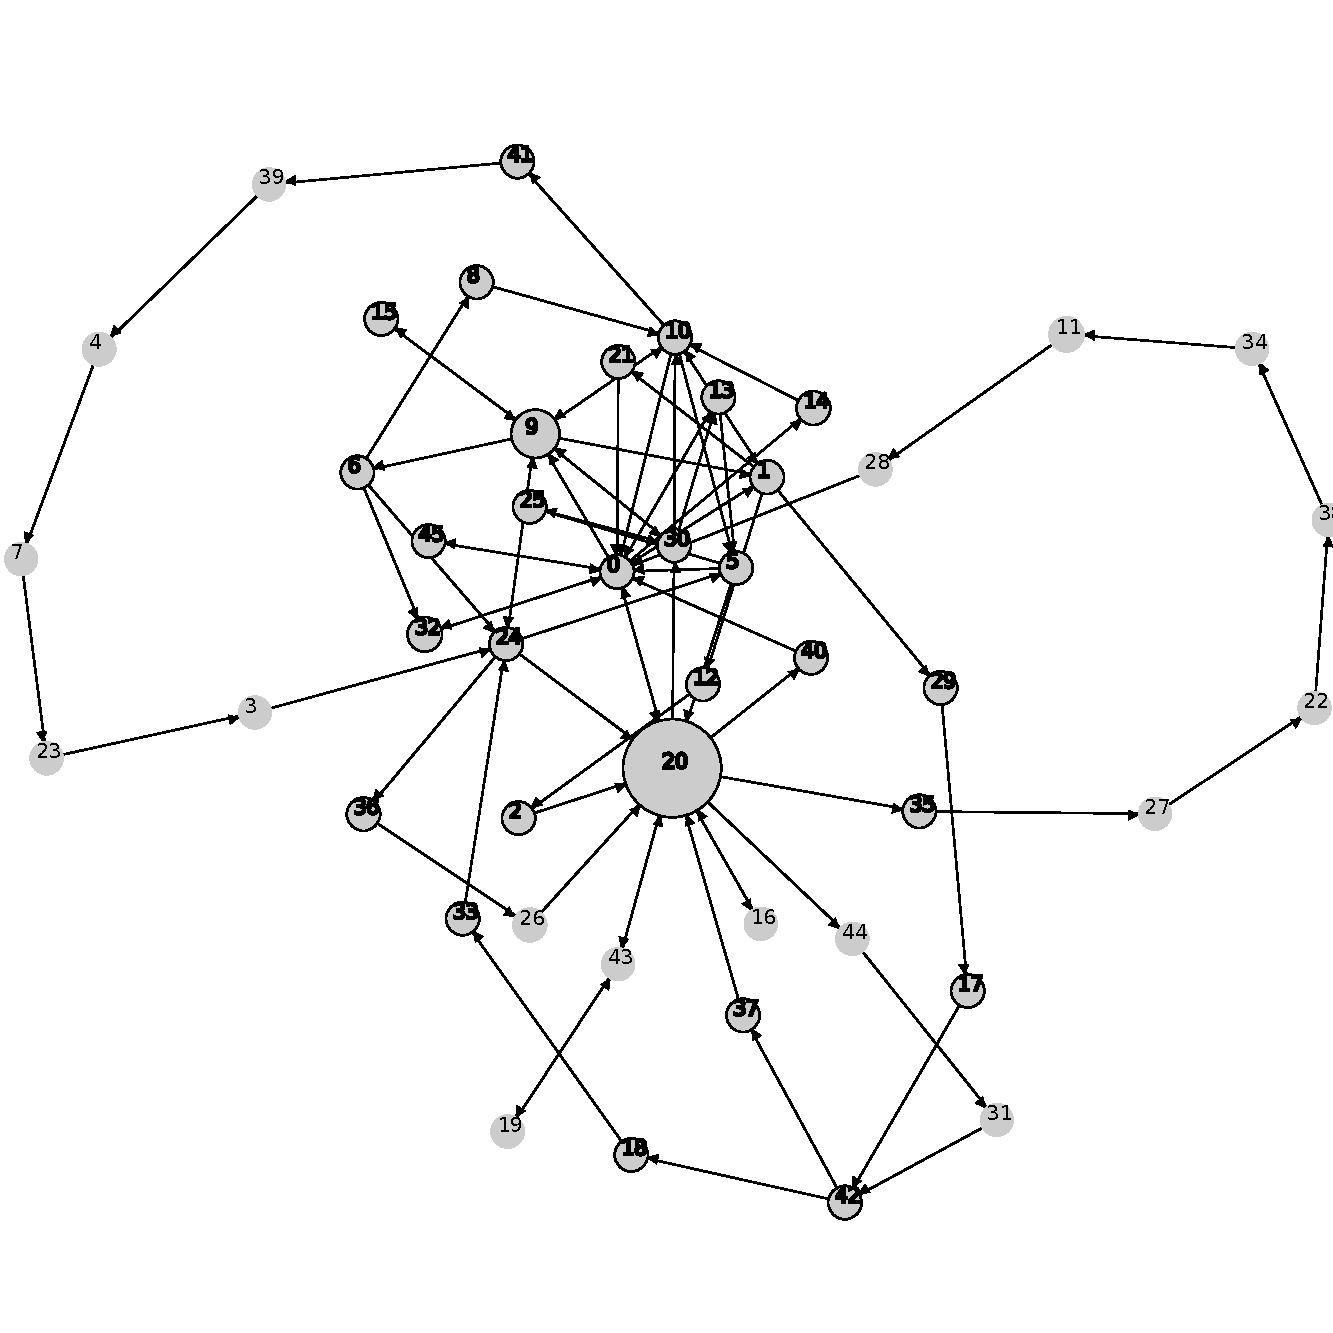
\includegraphics[width=4.5cm]{../plots/L0_filtered.pdf}
    }
    \subfigure[]{
        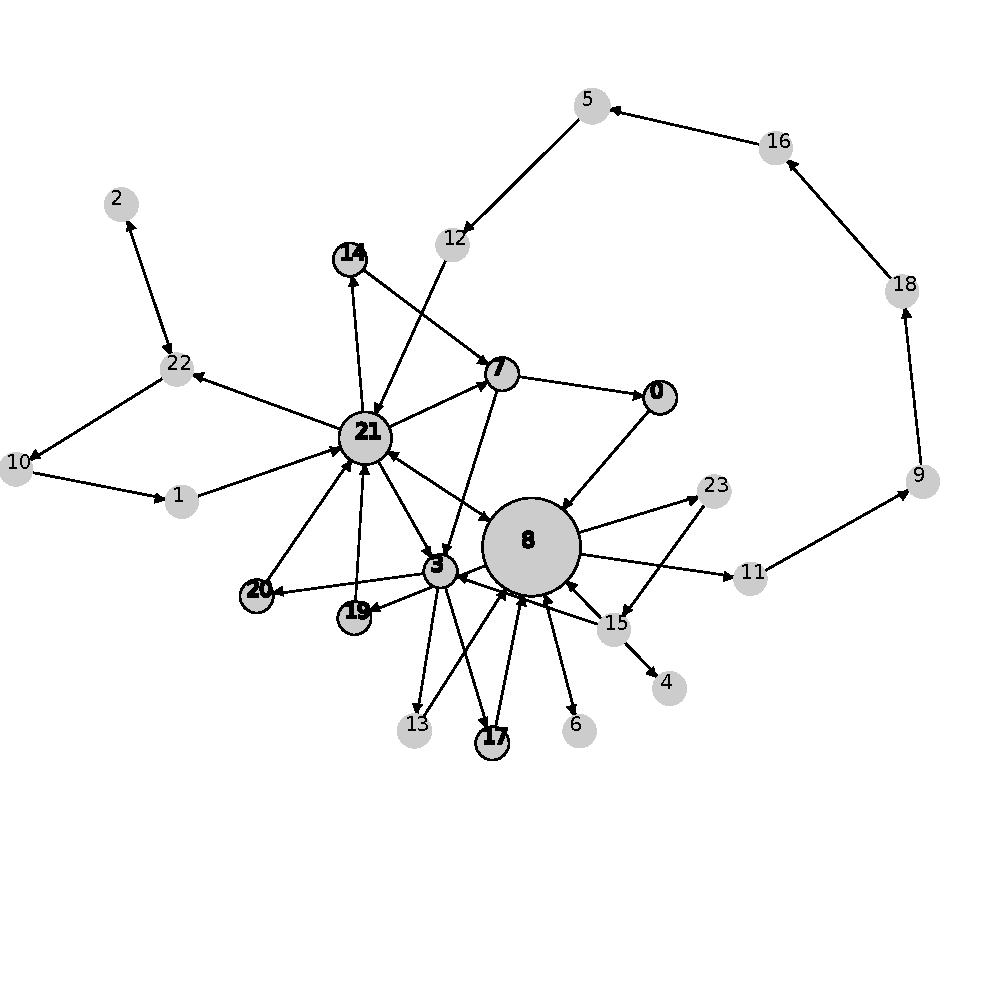
\includegraphics[width=4.5cm]{../plots/L1_filtered.pdf}
    }
    \subfigure[]{
        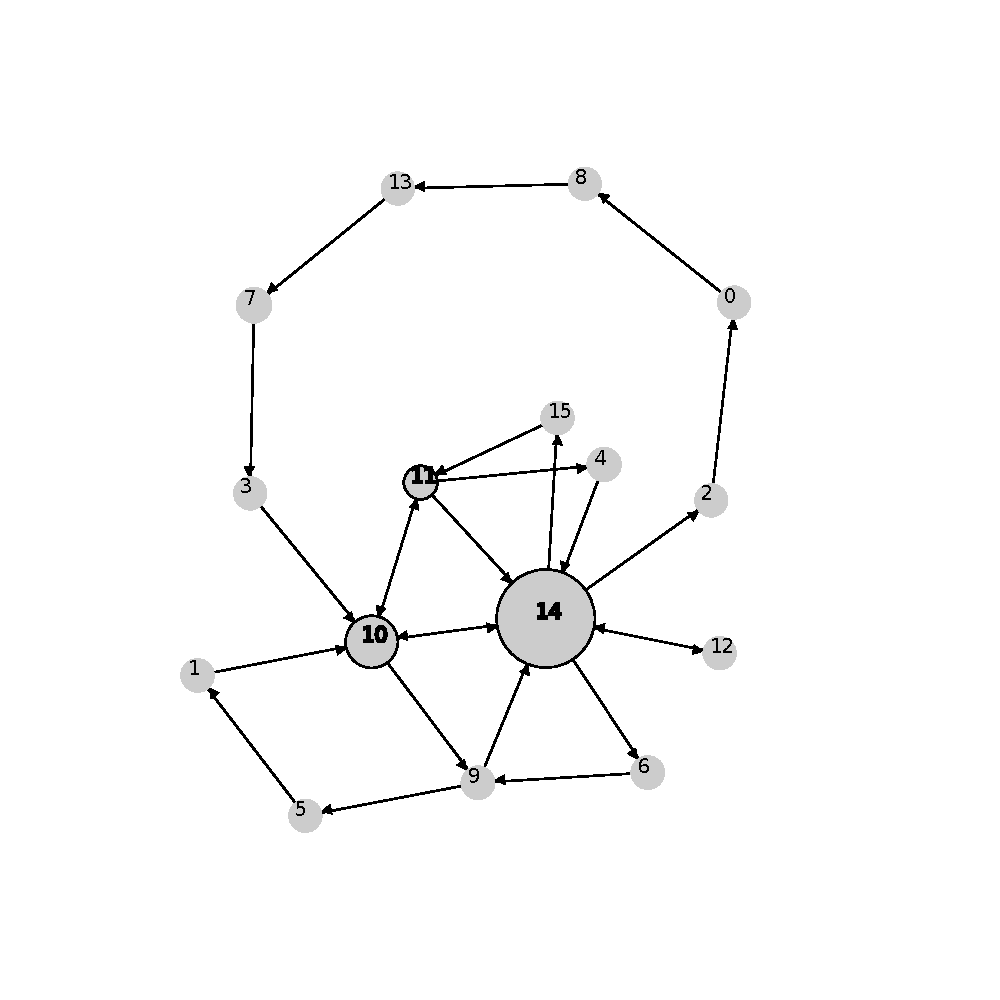
\includegraphics[width=4.5cm]{../plots/L2_filtered.pdf}
    }
    \caption{Transition diagrams of timelines of {\em persistent} locations labeled by: (a)
        physical locations, semantic labels with $i=2$, semantic labels with
        $i=1$.}
\end{figure*}

In Section~\ref{sec:movement} and Section~\ref{sec:loc}, we presented two online
algorithms $\mathbf{OnlineTimelineCluster}$ and $\mathbf{IdentifyLocations}$.
We compose the two algorithms forming a pipeline that automatically identifies
movements based on incoming WiFi hotspot readings.

The limitation of so far is that the algorithms have only been working with
BSSID signatures.  An example of a BSSID (for a Starbucks outlet) looks like 
{\tt 00:24:6c:46:c5:f0}.  Its use is limited to a universal identifier of the
WiFi hotspot, not as a humanly readable label.  For this reason, users can
assign semantically meaningful strings to BSSIDs.  For instance, {\tt
00:24:6c:46:c5:f0} is better known as ``{\tt Starbucks WiFi}" at this particular
location.

For the application of mobility analysis, SSID names are a valuable source of
semantic information about the physical location.  If two distinct physical
locations
both contain WiFi hotspots labeled by ``{\tt Startbucks Wifi}'' and ``{\tt
Starbucks Wifi 4893}'', then it is reasonable to infer that the mobile device
has visited two different coffee venues: both being {\tt Starbucks}, but at two
different physical locations.  
We would like to create succinct and informative
summarization of mobility in terms of semantically meaningful location groups to
the user by means of {\em semantic grouping} of locations.

By semantic grouping, we are to build a semantic location tree whose leaf nodes are the physical
locations, and the intermediate nodes are labeled.  An intermediate $x$ in the
location tree signify that the leaf nodes (physical locations) under $x$ are
semantically related.

Our assumption of semantic relevance is that
two WiFi hotpots are considered semantically related if they share some common
features in their user assigned SSID names.  For example, the {\tt
Starbucks4230} and {\tt Starbucks WiFi2039} share the common prefix of {\tt
Starbucks}.  This can be formalized by {\em semantic labels}.

\begin{definition}[Semantic labels of locations]
    Let $K = \{k_1, k_2, \dots, k_m\}$ be a set of keywords.
    We say that $K$ is can serve as a semantic label of a location $L$ if every
    keyword in $K$ is a prefix of a SSID label of WiFi hotspots of $L$.

    Namely,
    $$ \forall k\in K, \exists x\in\ssid(L), k\preceq x$$

    Two locations $L_1$ and $L_2$ are {\em mergable} by $K$ if $K$ is a semantic
    label for both $L_1$ and $L_2$.
\end{definition}

\begin{algorithm}[h]
    \begin{tabular}{|l|} \hline
        func SemanticMerge($\LL$, $n$) \\ 
        \RRR $\LL$: the list of locations \\
        \RRR $i$: the maximal of keywords to use as key \\ 
        \RRR {\em returns}: set of semantic locations \\ \hline
        $K^* = \mathrm{argmax} \{|\LL| - |\mathrm{merge}(\LL, K)| : K\in\ssid(\LL)^i\}$ \\
        $\delta = \mathrm{max} \{|\LL| - |\mathrm{merge}(\LL, K)| : K\in\ssid(\LL)^i\}$ \\
        while $\delta > 0$ \{ \\
        \RRR $\LL = \mathrm{merge}(\LL, K)$ \\
        \RRR $K^* = \mathrm{argmax} \{|\LL| - |\mathrm{merge}(\LL, K)| : K\in\ssid(\LL)^i\}$ \\
        \RRR $\delta = \mathrm{max} \{|\LL| - |\mathrm{merge}(\LL, K)| : K\in\ssid(\LL)^i\}$ \\
        \}\\
        return $\LL$ \\ \hline
    \end{tabular}
    \vspace{0.4cm}
    \caption{An algorithm to aggregate physical locations to groups based on
    their semantic information.}
    \label{alg:semantic}
\end{algorithm}



In the example of two locations containing SSID names of {\tt Starbucks4230} and
{\tt Starbucks WiFi2039} in their respective SSID sets, the keyword {\tt
Starbucks} can be used as part of a semantic label to represent both locations.

Given a semantic label, $K$, and a set of locations $\LL$, we can merge all the
locations $L\in \LL$ of which $K$ is a semantic label.  The merge function is
shown in Algorithm~\ref{alg:merge}.  The function {\tt merge($\LL$, $K$)} 
creates a new semantic location $L_\mathrm{new}$ that contains all the mergable
locations.

By building semantic locations using successively coarser keyword sets as
semantic labels, we can build a tree of semantic locations.

\begin{definition}[Semantic Location Tree]
    A {\em semantic location tree} is a tree with levels $0, 1, \dots n+1$, with leaf nodes at
    level 0 as the physical locations $\LL$.  At level $i>0$, the intermediate
    nodes are labeled by $n-i+1$ distinct names.
\end{definition}

For $n=3$, nodes at level 1 are labeled by $n-1+1=3$ distinct names.  At level
2, nodes are labeled by $n-2+1=2$ two distinct names.  The top-level is $n+1=4$,
which is labeled by $n-(n+1)+1 = 0$ names, so it has no labels.
The labels are used to reflect the commonality of the physical locations.
The root encompasses all the physical locations, and thus carries no semantic
labels.

At each level,  we iteratively merge locations using keyword sets of size
$i$.  We choose to select the keyword sets 
to maximize the reduction in the number of semantic locations after
merge.

Given a set of location $\LL$ with each location $L$ with a SSID set $\ssid(L)$,
the optimal semantic label $K*$ of length $i$ is defined as:

$$ K^* = \mathrm{argmax} \{|\LL| - |\mathrm{merge}(\LL, K)| : K\in\ssid(\LL)^i\}$$

The semenatic label $K^*$ is then used to merge the locations $\LL$ to $\LL'$.  We then
iteratively pick the optimal semantic label of $\LL'$, and repeat the merge
step.  The iteration terminates if $K^*$ can no reduce the number of locations.
This is formally described in Algorithm~\ref{alg:semantic}.

\section{Implementation and Experimental Evaluation}

\begin{figure}[t]
    \centering
    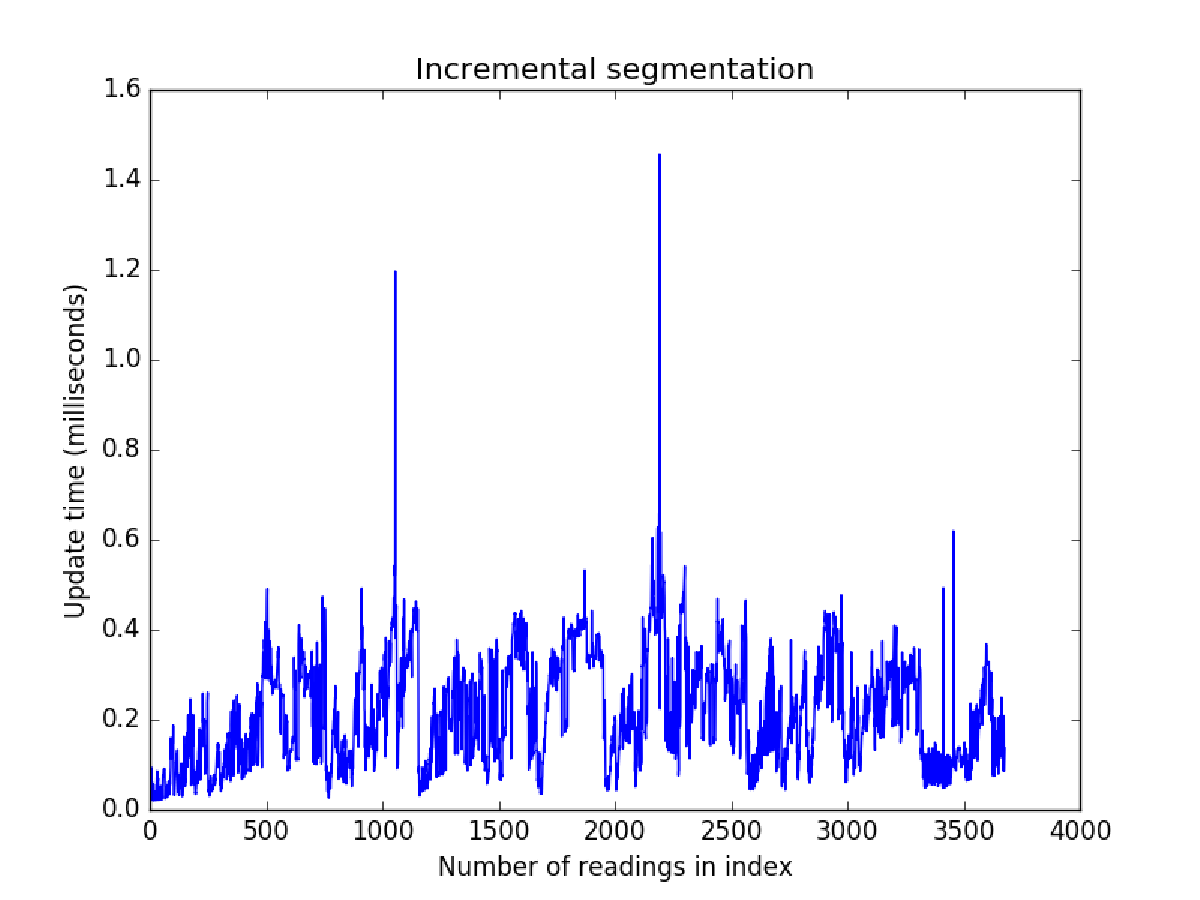
\includegraphics[width=3.5in]{../plots/incremental.pdf}
    \caption{Performance of the online location identification}
    \label{fig:incremental}
\end{figure}
